\chapter{Overview of current approaches}
\label{chap:overview}

\changed{This chapter surveys how the (M)RCPSP is solved in the literature
and identifies the gap the proposed algorithm addresses. It first
introduces the schedule generation schemes and the solution representation
that virtually every heuristic for the problem shares
(Section~\ref{sec:rcpsp-formalization}), then evolutionary algorithms and
genetic programming (Section~\ref{sec:ea-metaheuristics}), and finally the
existing exact and metaheuristic approaches together with the research gap
(Section~\ref{sec:existing-approaches}).}

%==============================================================================
\section{\texorpdfstring{\changed{Schedule generation schemes and solution representation}}{Schedule generation schemes and solution representation}}
\label{sec:rcpsp-formalization}
%==============================================================================

\changed{This section introduces the schedule generation scheme used by
almost every (M)RCPSP heuristic to decode priorities into feasible
schedules, and connects it to solution representation, continuing the
worked example of Table~\ref{tab:example} under an added resource
constraint.}

\subsection{Schedule generation schemes}
\label{subsec:sgs}

Constraint~\eqref{eq:rcpsp-res} cannot be resolved by a single forward pass: at
any point several activities may be precedence-eligible while only some of them
fit within the remaining resource capacity. Almost every constructive heuristic
and every metaheuristic for the RCPSP therefore builds a schedule with a
\emph{schedule generation scheme} (SGS), a step-wise procedure that, at each
step, chooses one eligible activity from a \emph{decision set} and fixes its
start time so that~\eqref{eq:rcpsp-res} stays satisfied, until every activity is
scheduled~\cite{kolisch1996sgs}. The two classical variants differ in their
decision set:
\begin{description}
  \item[Serial SGS] processes activities one at a time. At each step the decision
        set $D$ contains every unscheduled activity whose predecessors are
        already scheduled; one activity is selected from $D$ (by a priority
        rule, see below) and given the earliest start time that respects both
        precedence and the resource capacities given everything scheduled so
        far. Serial SGS always reaches a so-called \emph{active} schedule:
        \changed{one in which no activity can be started earlier without delaying
        some other activity or violating a constraint. This matters because
        the set of active schedules is guaranteed to contain an optimal
        solution, so restricting the search to them loses
        nothing~\cite{kolisch1996sgs}.}
  \item[Parallel SGS] advances a clock $t$ instead of an activity counter. At
        each decision point $t$ it forms the set of all activities that are
        precedence-eligible \emph{and} resource-feasible at $t$, schedules as
        many of them as the remaining capacity allows (again by priority), and
        then advances $t$ to the next finish time.
\end{description}
Kolisch's empirical comparison of the two schemes is more nuanced than the
active-schedule argument alone suggests: in single-pass mode parallel SGS
actually attains a \emph{lower} average deviation from the optimum than
serial SGS, and under biased random sampling serial SGS only pulls ahead for
larger sample sizes and moderately resource-constrained instances, with
parallel SGS remaining competitive for small samples and tightly constrained
instances~\cite{kolisch1996sgs}. This thesis nonetheless adopts serial SGS as
the default decoding procedure throughout, since it alone is guaranteed to
reach the active-schedule space containing the optimum (the argument above),
with the parallel variant reserved for the dual-decoding experiments of
Chapter~\ref{chap:approach}. \changedB{Algorithms~\ref{alg:parallel-sgs}
and~\ref{alg:serial-sgs} state the two variants in full, each driven by a
generic priority rule $\pi$; Chapter~\ref{chap:approach} instantiates the
serial variant with the evolved rule pair that drives it in this thesis.}

\begin{algorithm}[htbp]
\caption[Parallel SGS with a priority rule]{\changed{Parallel SGS with a
priority rule $\pi$ (lower value = higher priority).}}
\label{alg:parallel-sgs}
\begin{algorithmic}[1]
\Require instance with activities $V$; priority rule $\pi$
\State $t \gets 0$;\quad $S \gets \emptyset$ \Comment{clock and scheduled set}
\While{$S \neq V$}
  \State $D_t \gets \{\, j \in V \setminus S : \text{all predecessors of } j$
    \Statex \hspace{\algorithmicindent}\hspace{\algorithmicindent}
    $\text{finished by } t \text{ and } j \text{ resource-feasible at } t \,\}$
  \While{$D_t \neq \emptyset$}
    \State $j^{*} \gets \arg\min_{j \in D_t} \pi(j)$; start $j^{*}$ at time $t$;
      $S \gets S \cup \{j^{*}\}$
    \State recompute $D_t$ under the reduced remaining capacity at $t$
  \EndWhile
  \State $t \gets$ the earliest finish time of a running activity after $t$
\EndWhile
\State \Return the completed schedule
\end{algorithmic}
\end{algorithm}

\begin{algorithm}[htbp]
\caption[Serial SGS with a priority rule]{\changedB{Serial SGS with a
priority rule $\pi$ (lower value = higher priority).}}
\label{alg:serial-sgs}
\begin{algorithmic}[1]
\Require instance with activities $V$; priority rule $\pi$
\State $S \gets \emptyset$ \Comment{already-scheduled activities}
\While{$S \neq V$}
  \State $D \gets \{\, j \in V \setminus S : \text{all predecessors of } j \text{ are in } S \,\}$ \Comment{decision set}
  \State $j^{*} \gets \arg\min_{j \in D} \pi(j)$
  \State start $j^{*}$ at the earliest time respecting precedence and
    resource capacities
  \State update remaining resource availabilities; $S \gets S \cup \{j^{*}\}$
\EndWhile
\State \Return the completed schedule
\end{algorithmic}
\end{algorithm}

\subsection{Solution representation: from chromosomes to schedules}
\label{subsec:representation-intro}

An SGS by itself only decides feasibility; it needs a \emph{priority value} for
every activity in the decision set to break ties between simultaneously
eligible activities. The classical representation, going back to the first
genetic algorithms for the RCPSP~\cite{hartmann1998}, encodes a solution as an
\emph{activity list}: a permutation of $V$ that respects all precedence
relations (a topological order of the activity network). Decoding such a
chromosome with one pass of the serial SGS (always select, from the current
decision set, the eligible activity that appears earliest in the list) yields
exactly one feasible schedule for exactly one problem instance. This
representation-then-decoding split, chromosome on one side and SGS on the
other, is what later allows genetic \emph{programming} to replace the
chromosome with a reusable priority \emph{rule}, as
Section~\ref{sec:ea-metaheuristics} develops.

\subsubsection*{Worked example, continued}

Table~\ref{tab:example} introduced six activities with no resource constraints;
Figure~\ref{fig:cpm-network} found a makespan of 15. Suppose now a single
renewable resource $R$ of capacity 2 is added, with per-activity demands
$r_A=1,\, r_B=2,\, r_C=1,\, r_D=2,\, r_E=1,\, r_F=1$. The unconstrained schedule
of Figure~\ref{fig:gantt-slack} is no longer resource-feasible, since it runs
$B$ and $C$ concurrently from $t=3$ to $t=5$, a combined demand of $1+2=3 > 2$.
Decoding the activity-list chromosome $[A, C, E, B, D, F]$ with the serial SGS of
Section~\ref{subsec:sgs} resolves the conflict: $A$ and $C$ are scheduled as
before, but $B$, although precedence-eligible from $t=3$, right after $A$
finishes, cannot start until $t=7$, because at any earlier time its demand of
2 units would push the combined usage with the still-active $C$ or $E$ above
the capacity of 2. Only once $C$ and $E$ have both finished does enough capacity
free up. Activities $D$ and $F$ then simply follow in precedence order, giving
the schedule and Gantt chart of Figure~\ref{fig:sgs-decoding} and a makespan of
19: four time units above the unconstrained CPM value, a gap attributable
entirely to resource contention rather than precedence.

\begin{figure}[htbp]
  \centering
  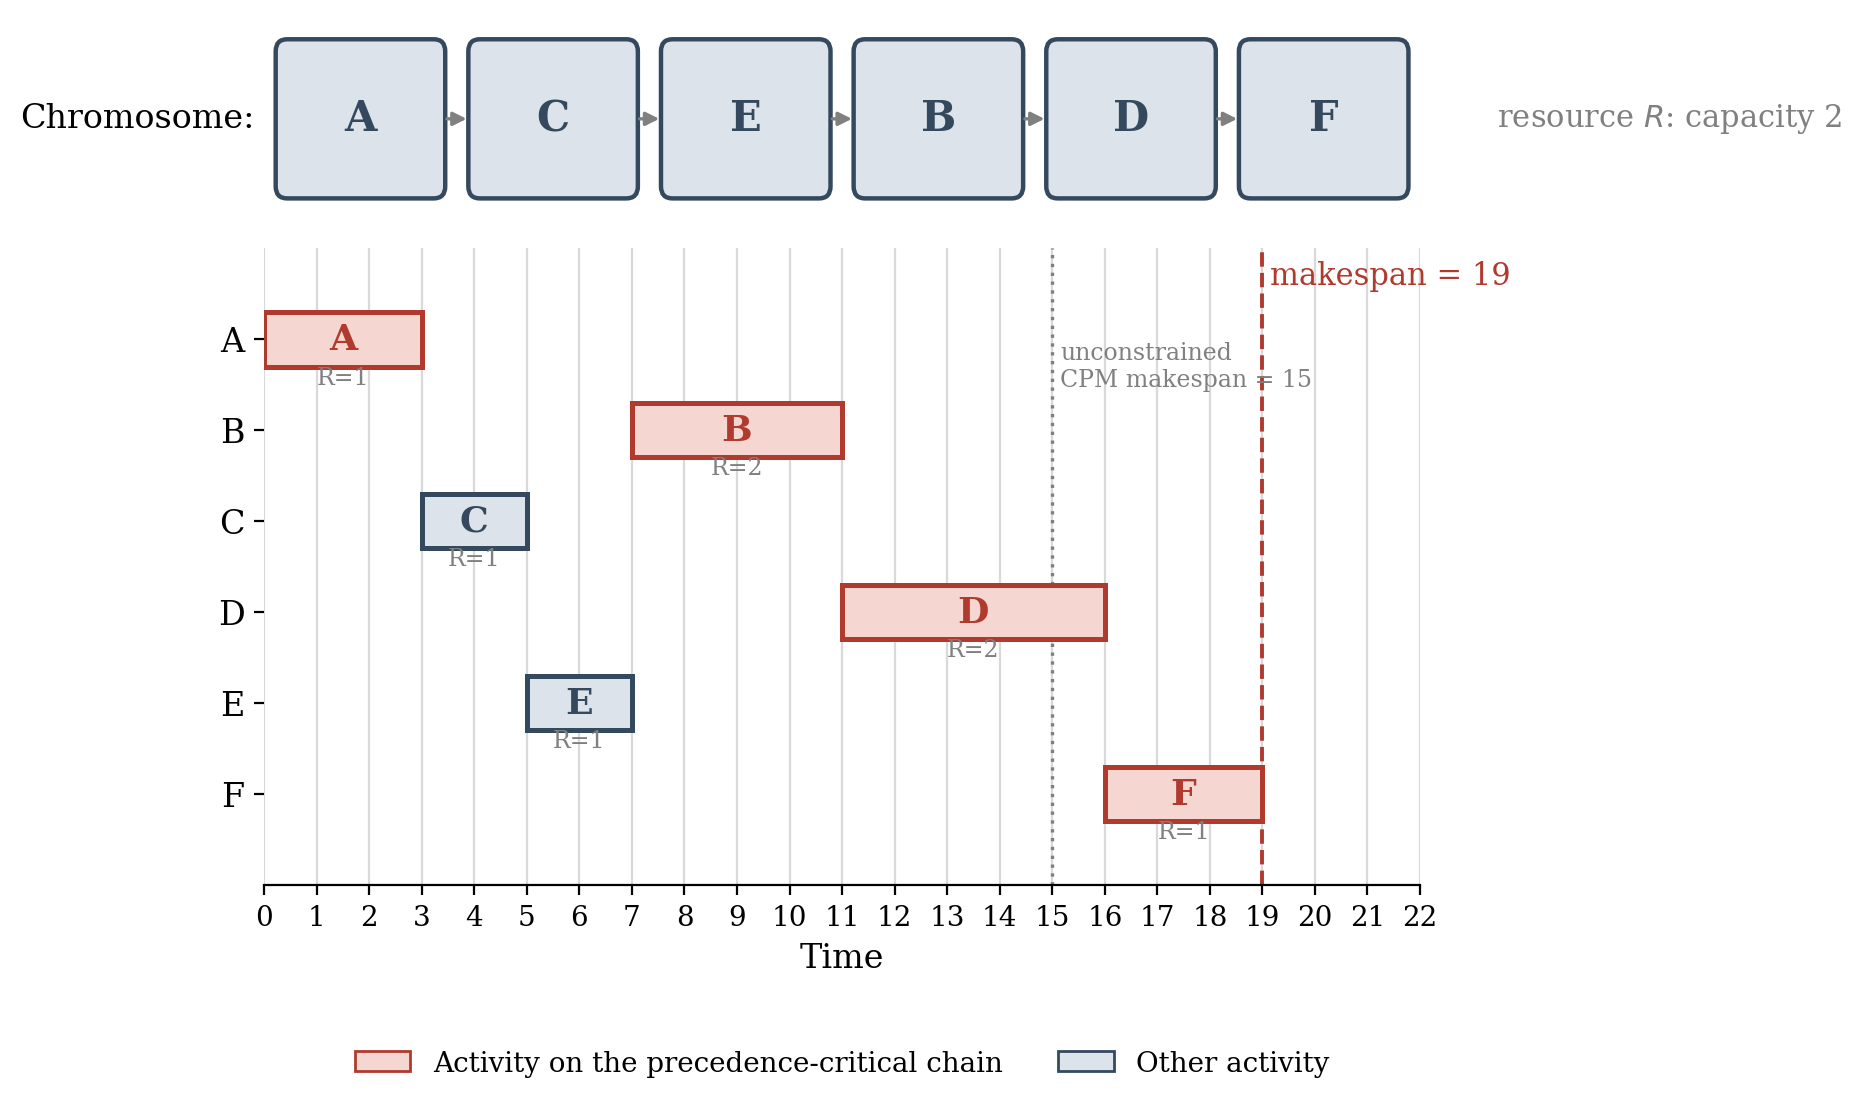
\includegraphics[width=\textwidth]{img/sgs-decoding.png}
  \caption[Serial SGS decoding under a resource constraint]{Decoding the
  activity-list chromosome $[A,C,E,B,D,F]$ with the serial SGS, under a single
  renewable resource $R$ of capacity 2 (demands shown below each bar). Activity
  $B$ is delayed from its precedence-eligible time $t=3$ to $t=7$ by resource
  contention with $C$ and $E$; the resulting makespan is 19, against the
  unconstrained CPM value of 15 (Figure~\ref{fig:gantt-slack}).}
  \label{fig:sgs-decoding}
\end{figure}

%==============================================================================
\section{Evolutionary algorithms and metaheuristics}
\label{sec:ea-metaheuristics}
%==============================================================================

\changed{This section introduces the algorithmic family on which the rest of the
thesis builds: the evolutionary loop shared by every such algorithm, and
the two representations relevant here, the fixed-length chromosome of a
genetic algorithm and the variable-size program tree of genetic
programming.}

\subsection{The general evolutionary loop}
\label{subsec:ea-loop}

An evolutionary algorithm (EA) maintains a \emph{population} of candidate
solutions, called individuals, and repeatedly applies three biologically
inspired operators to it: \emph{selection} favours individuals with better
fitness as parents; \emph{variation} (crossover and mutation) produces offspring
by recombining or perturbing parents; and \emph{replacement} forms the next
generation from parents and offspring, usually again biased toward
fitness. No assumption is made about the objective being
convex, differentiable, or even computable in closed form, only that
candidate solutions can be evaluated and compared, which is precisely why EAs
remain effective on a combinatorially structured, discontinuous landscape such
as the RCPSP makespan surface described in
Section~\ref{sec:challenges}~\cite{dokeroglu2025metaheuristics}.
Figure~\ref{fig:ea-loop} depicts this cycle.
What changes between EA \emph{families} is the representation of an
individual and the variation operators defined on it; the next two subsections
contrast the two representations relevant to this thesis.

\begin{figure}[htbp]
  \centering
  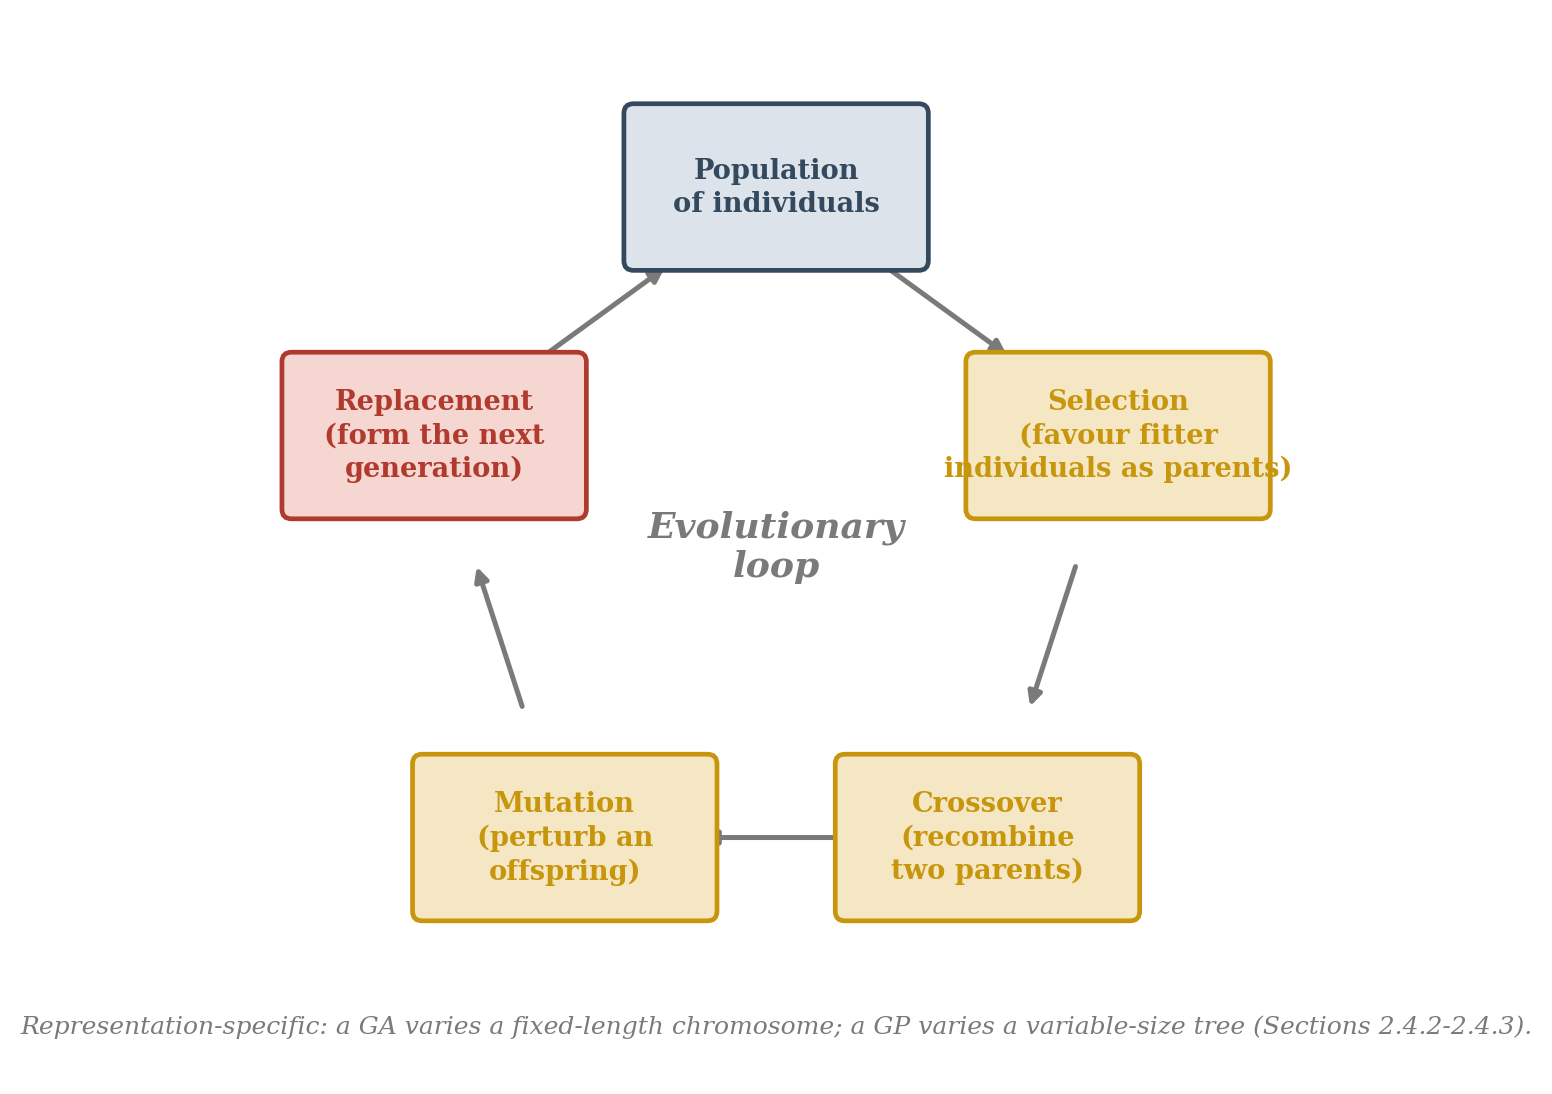
\includegraphics[width=0.72\textwidth]{img/ea-loop.png}
  \caption[The general evolutionary loop]{The general evolutionary loop
  shared by every EA family discussed in this thesis: selection biases which
  individuals become parents, crossover and mutation jointly form the
  variation step that produces offspring, and replacement assembles the next
  generation. Sections~\ref{subsec:ga-rcpsp} and~\ref{subsec:gp-hh} keep this
  loop fixed and contrast only the representation on which crossover and
  mutation operate.}
  \label{fig:ea-loop}
\end{figure}

\subsection{Genetic algorithms for (M)RCPSP}
\label{subsec:ga-rcpsp}

A genetic algorithm (GA) represents each individual as a fixed-length
chromosome over a finite alphabet, classically a bit string, and applies
generic operators such as one-point crossover or bit-flip mutation defined
purely on that encoding. Applied to the RCPSP, the
chromosome is the activity-list permutation of
Section~\ref{subsec:representation-intro}, possibly paired with a
mode-assignment list for the multi-mode case; specialised operators such as
precedence-preserving crossover keep every offspring chromosome a valid
topological order~\cite{hartmann1998,hartmann2002}. Decoding with the serial SGS
of Section~\ref{subsec:sgs} converts the chromosome into a fitness value (the
makespan); Van Peteghem and Vanhoucke's GA for the preemptive and
non-preemptive MRCPSP, and its extension to a wide instance set, established
this activity-list-plus-SGS design as the standard GA baseline for the multi-mode
problem~\cite{vanpeteghem2010,vanpeteghem2014}. Crucially, the chromosome
\emph{is} the schedule of one specific instance: evolving a population means
searching for one good solution, and the search must restart from scratch for
every new project.

\subsection{Genetic programming and hyper-heuristics}
\label{subsec:gp-hh}

Genetic programming (GP), introduced by Koza as a way of \changedB{evolving} computer
programs rather than fixed-length strings~\cite{koza1994gp}, keeps the
evolutionary loop of
Section~\ref{subsec:ea-loop} but replaces the fixed-length chromosome with a
variable-size syntax tree, typically representing an arithmetic or logical
expression: internal nodes are \emph{functions} (e.g. $+, -, \min$) and leaves
are \emph{terminals} (input features or constants).
Subtree crossover exchanges randomly chosen subtrees between two parent trees,
and subtree mutation replaces a subtree with a freshly generated random one;
because every well-formed subtree is itself a well-formed tree, these operators
need no special repair mechanism to stay closed under the representation.

When a GP tree is interpreted not as a direct solution but as a \emph{priority
rule} (compiled once and then queried by an SGS every time it must break a tie
in the decision set), the result is a \emph{genetic-programming
hyper-heuristic} (GPHH): instead of searching for one schedule, the algorithm
searches for one re-usable rule that an SGS can apply to \emph{any} instance of
the problem class~\cite{branke2016gphh}.
Figure~\ref{fig:representation-contrast} contrasts the two representations
directly: the GA chromosome of Section~\ref{subsec:ga-rcpsp} decodes, with one
SGS pass, into a single schedule for a single instance, whereas a GP tree such
as $\min(\mathrm{LST},\, \mathrm{GRPW} - \mathrm{Duration})$ is compiled into a
priority function that an SGS can query on an unseen instance without any
further evolution. This shift from instance-specific solutions to
generalisable rules is what makes GPHH attractive whenever many related
instances must be solved repeatedly, exactly the setting evaluated in
Chapter~\ref{chap:experiments}, and it is the representation adopted by the
baseline of this thesis~\cite{Tian2024GPHH}.

\begin{figure}[htbp]
  \centering
  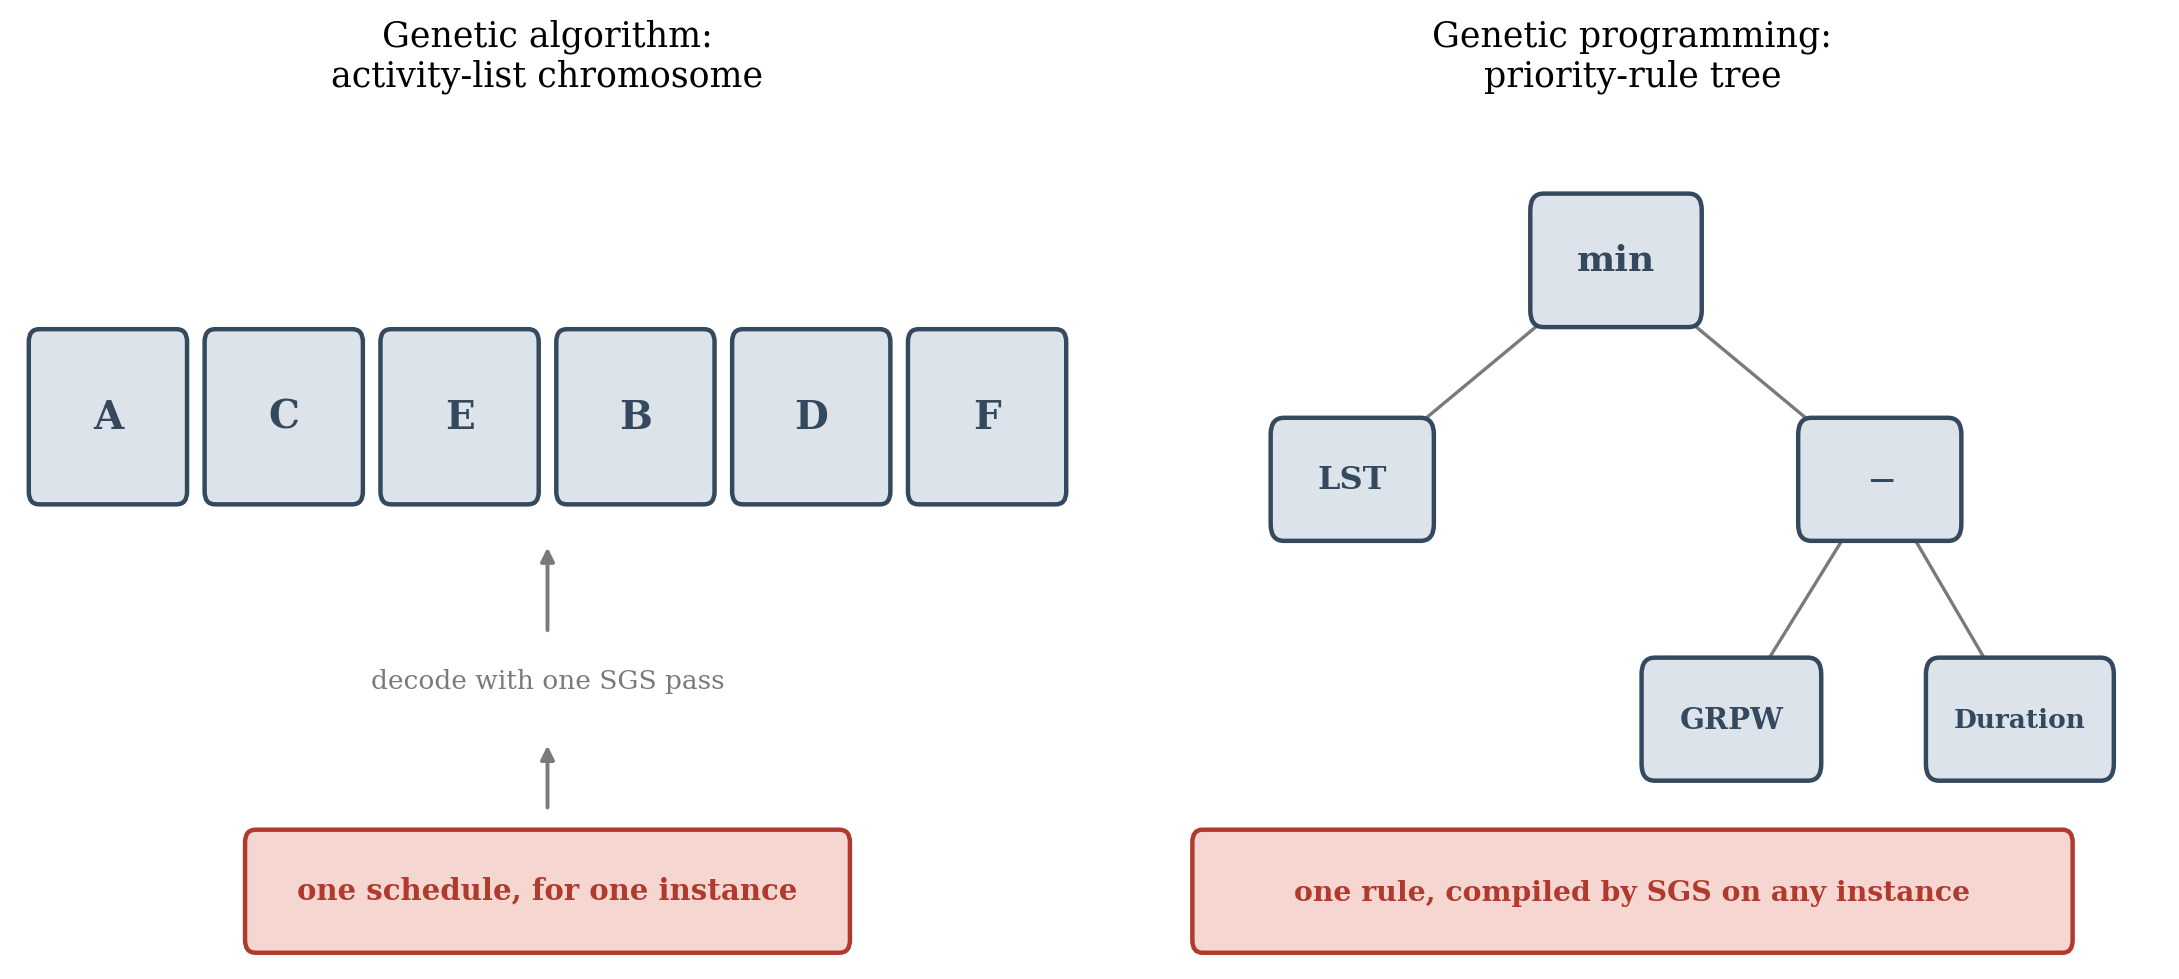
\includegraphics[width=0.92\textwidth]{img/representation-contrast.png}
  \caption[GA chromosome vs.\ GP priority-rule tree]{The representation
  contrast between a genetic algorithm and a genetic-programming
  hyper-heuristic. The GA chromosome decodes, via one SGS pass, into a schedule
  for one instance; the GP tree is a priority rule that an SGS can compile and
  apply to any instance of the problem class.}
  \label{fig:representation-contrast}
\end{figure}

%==============================================================================
\section{Existing approaches for (M)RCPSP}
\label{sec:existing-approaches}
%==============================================================================

\changed{This section surveys how the literature has actually solved the (M)RCPSP,
moving from exact methods through metaheuristics and local search to the
genetic-programming hyper-heuristics most directly related to this thesis,
and closes with the specific gap that Chapter~\ref{chap:approach}
addresses.}

\subsection{Exact methods}
\label{subsec:exact}

Exact algorithms for the MRCPSP are almost exclusively branch-and-bound
procedures that explore the space of precedence- and resource-feasible partial
schedules, pruned with lower bounds derived from the (mode-relaxed) critical
path; this style of bounding remains the reference point for newer exact
formulations, e.g. for the generalized-precedence
MRCPSP/max~\cite{bartusch1988}. Because the underlying decision problem is
NP-complete (Section~\ref{subsec:mrcpsp-model}), these methods scale to at most
a few dozen activities before running times become impractical, which is the
chief reason that metaheuristics dominate the literature for realistically sized
instances~\cite{demeulemeester2002,hartmann2010survey}. Recent work narrows
this gap from two directions rather than closing it outright: Chakrabortty,
Sarker and Essam reduce the variable count of event-based \changed{mixed-integer
linear programming (MILP)} formulations
for the MRCPSP~\cite{chakrabortty2014event}, while Vanhoucke and Coelho
combine branch-and-bound with metaheuristic-style restriction of the search
space in a matheuristic that reports new best-known solutions on standard
RCPSP benchmarks~\cite{vanhoucke2024matheuristic}, building on their earlier
result that the feasible solution space of an RCPSP instance can itself be
reduced without excluding any optimum~\cite{vanhoucke2024reducing}. Neither
line of work scales to the MMLIB50/MMLIB100 instance sizes used in this
thesis (Chapter~\ref{chap:dataset}).

\subsection{Classical and recent metaheuristics}
\label{subsec:metaheuristics}

Besides the genetic algorithms already discussed in
Section~\ref{subsec:ga-rcpsp}, the RCPSP and MRCPSP have been attacked with
essentially every major metaheuristic framework: simulated annealing, tabu
search, scatter search, ant colony optimisation and particle swarm
optimisation, each paired with the activity-list-plus-SGS encoding of
Section~\ref{subsec:representation-intro} and a framework-specific notion of
neighbourhood or pheromone update~\cite{kolisch2006,khajesaeedi2025review}.
Table~\ref{tab:recent-approaches} samples how active this line of work remains:
Peng et al.~\cite{peng2023quantumpso}
hybridise quantum-behaved particle swarm optimisation with the JAYA search
operator for a multi-skill multi-mode variant; and Cai, Bian and
Liu~\cite{cai2024rlgnn} depart from population-based search altogether, training
a graph-neural-network policy with proximal policy optimisation to schedule
under resource disruptions. Mirror-based and hybrid differential-evolution
GAs continue to be proposed for the plain MRCPSP itself: Zamani's mirror GA
solves an instance and a mode-inverted counterpart in parallel and reports
results competitive with or better than earlier GA baselines on PSPLIB and
MMLIB~\cite{zamani2019mirror}, and Cheng and Tran combine chaotic search with
fuzzy $c$-means clustering in a differential-evolution algorithm specifically
to avoid the premature convergence that plagues simpler
GAs~\cite{cheng2016fcde}. Priority-rule design itself also remains an active
topic in its own right: Buddhakulsomsiri and Kim extend priority-rule
heuristics with resource vacations and activity
splitting~\cite{buddhakulsomsiri2007}, and Adamu, Okagbue and Oguntunde
combine several classical rules into a single hybrid rule via machine
learning~\cite{adamu2019priority}, both hand-designing exactly the kind of
composite priority function that the GP of Chapter~\ref{chap:approach}
instead evolves automatically. Across this diversity, the encoding and decoding
machinery of Sections~\ref{subsec:representation-intro}
and~\ref{subsec:ga-rcpsp} is shared almost universally; what differs is how
candidate priority lists are proposed and accepted.

\begin{table}[htbp]
  \centering
  \caption[Representative metaheuristic approaches for (M)RCPSP]{\changed{Representative
  metaheuristic approaches for (M)RCPSP, in
  chronological order, illustrating the range of frameworks (swarm,
  local-search, learning-based and evolutionary) applied to the problem.}}
  \label{tab:recent-approaches}
  \begin{tabularx}{\textwidth}{@{}>{\raggedright\arraybackslash}X >{\raggedright\arraybackslash}p{3.1cm} >{\raggedright\arraybackslash}X c@{}}
    \toprule
    \textbf{Method} & \textbf{Reference} & \textbf{Problem variant} & \textbf{Year} \\
    \midrule
    Fuzzy-clustering chaotic DE & Cheng and Tran~\cite{cheng2016fcde} & Multi-mode & 2016 \\
    Mirror-based GA & Zamani~\cite{zamani2019mirror} & Multi-mode & 2019 \\
    MILP, weighted earliness/tardiness & Ruhlusara\c{c} and \c{C}al{\i}\c{s}kan~\cite{ruhlusarac2022dynamic} & Dynamic, multi-mode, multi-project & 2022 \\
    Hybrid quantum PSO & Peng et al.~\cite{peng2023quantumpso} & Multi-skill, multi-mode & 2023 \\
    Multi-start iterated local search & Ramos et al.~\cite{ramos2023stochastic} & Stochastic, multi-mode & 2023 \\
    RL with graph neural network & Cai et al.~\cite{cai2024rlgnn} & Resource disruptions & 2024 \\
    NSGA-II + $Q$-learning & Yang et al.~\cite{yang2024biobjective} & Multi-objective, multi-project & 2024 \\
    Hybrid differential evolution & van der Beek et al.~\cite{VanDerBeek2024} & Flexible project structure & 2024 \\
    Two-tree GPHH (this thesis' baseline) & Tian et al.~\cite{Tian2024GPHH} & Multi-mode & 2024 \\
    Multi-tree GP, knee-point grouping & Tian et al.~\cite{tian2025multitree} & Dynamic, multi-mode & 2025 \\
    \bottomrule
  \end{tabularx}
\end{table}

\subsection{Local search and schedule improvement}
\label{subsec:local-search}

Orthogonal to how a priority list is searched is how the schedule it decodes
into can be \emph{improved after the fact}, without changing the underlying
list. The best-known such technique is \emph{justification}: starting from a
schedule built by a forward SGS, a backward pass right-justifies every
activity (delays it as late as possible without increasing the makespan), and a
further forward pass left-justifies the result again; Valls, Ballest{\'i}n and
Quintanilla show that this single- or double-justification step is
computationally cheap and, applied across more than twenty published RCPSP
algorithms on the PSPLIB j120 benchmark, never worsened a schedule while
improving the large majority of
cases~\cite{valls2005justification}. \changed{The reason it works is that each pass
moves every activity as far as it can go in one direction without extending
the project: right-justification compacts the schedule against its end and
thereby frees resource capacity early on, and the subsequent
left-justification can exploit those freed periods to start activities
earlier than the original schedule allowed; since no activity is ever moved
past the current makespan, the makespan can only stay equal or decrease.}
Because justification operates purely on the
decoded schedule, it composes with \emph{any} priority-list search method,
genetic or otherwise, and Chapter~\ref{chap:approach} revisits it directly as
one of the operators evaluated for the algorithm proposed in this thesis.
A related idea is to plan \emph{bidirectionally} from the outset rather than
improving a forward schedule afterwards: Klein embeds backward,
deadline-oriented scheduling passes directly into priority-rule heuristics and
reports substantial makespan improvements over forward-only
scheduling~\cite{klein2000bidirectional}, a precedent that
Chapter~\ref{chap:approach} revisits not for a single priority-list heuristic
but for an evolved GPHH rule, via the backward serial SGS introduced there.
Closer still to the multi-mode setting of this thesis, Afshar, Shahhosseini
and Sebt pair a standard GA with a purpose-built local search operator for
the MRCPSP specifically, and report consistent makespan improvements over
the GA alone across PSPLIB instances~\cite{afshar2022ga}; their result is
direct evidence, for this thesis's own problem variant rather than a
related one, that a local, schedule-level refinement step can improve on a
population-based search's own output, the same motivation
Section~\ref{subsec:localsearch-eval} gives for pairing critical-path local
search with the GPHH baseline.

\subsection{Hyper-heuristics and genetic-programming-based scheduling}
\label{subsec:gphh-related}

The GPHH idea introduced in Section~\ref{subsec:gp-hh} has its own substantial
literature, anchored by the foundational review of
Branke et al.~\cite{branke2016gphh} and, more generally, by Burke, Hyde,
Kendall and Woodward's demonstration that GP can automate heuristic design
across many combinatorial domains, not just scheduling~\cite{burke2012automating}.
Early applications to the (single-mode) RCPSP itself compared a GA directly
against a single-tree GP priority rule: Frankola, Golub and Jakobovi\'c note
that, unlike a GA chromosome, an evolved GP rule transfers to instances unseen
during search and is therefore better suited to dynamic
environments~\cite{frankola2008evolutionary}, and \DJ umi\'c, \v{S}i\v{s}ejkovi\'c,
\v{C}ori\'c and Jakobovi\'c develop a systematic terminal-selection methodology
for the same single-tree setting~\cite{dumic2018evolving}; neither extends to
the additional non-renewable-resource and mode-selection decisions that the
multi-mode problem requires. Most applications still target (dynamic) job-shop
and flow-shop scheduling rather than project scheduling: Zhang, Mei and
Zhang's factored GP representation for dynamic flexible job-shop scheduling,
which multiplies a fixed, hand-designed sub-expression with a freely evolved
one, is a representative example of how this wider literature engineers GP
representations~\cite{zhang2019new}. Within project scheduling specifically,
the GPHH of Tian, Mei and Zhang adapted to the MRCPSP and adopted as the
baseline of this thesis evolves two cooperating trees, one priority rule for choosing the next activity
and one for choosing its execution mode, decoded jointly by the serial
SGS~\cite{Tian2024GPHH}. The same authors' most recent
follow-up~\cite{tian2025multitree} extends the multi-tree design with a
knee-point-guided activity-group selection mechanism for the \emph{dynamic}
multi-mode problem, confirming, together with a recent survey of the
broader project-scheduling field~\cite{servranckx2024preface}, that
multi-tree GPHH for the MRCPSP is an active and still-evolving research
direction rather than a closed topic.

\subsection{Research gap}
\label{subsec:research-gap}

Three observations from this survey motivate the approach taken in
Chapter~\ref{chap:approach}. First, and most directly, the GPHH baseline of
Tian, Mei and Zhang~\cite{Tian2024GPHH} gives its evolved priority rule
terminals describing precedence structure and renewable-resource demand,
but nothing about non-renewable resource state, even though mode choice is
exactly the decision that trades duration and renewable-resource use
against non-renewable consumption. To the best of our knowledge, no
published GPHH for the MRCPSP exposes non-renewable budget information to
the evolving rule directly. Second, the local-search literature
(Section~\ref{subsec:local-search}) and the GPHH literature
(Sections~\ref{subsec:gp-hh}--\ref{subsec:gphh-related}) have developed
almost independently: schedule-level refinement techniques such as
justification are applied routinely to GA-evolved schedules but, to the
best of our knowledge, rarely to the schedules produced by a GPHH-evolved
rule, leaving open whether a \changed{schedule-level local-search} refinement step
benefits an evolved priority rule the way it benefits a directly-evolved
schedule. Third, the
GP literature's own selection-mechanism alternatives to tournament
selection, epsilon-lexicase selection among them, have seen comparatively
little systematic evaluation on multi-instance scheduling rules
specifically, despite selection pressure being a mechanism that can be
changed without touching representation or fitness at all. Chapter~\ref{chap:approach}
accordingly proposes closing the first gap directly, with non-renewable
resource terminals, and screens the second and third empirically, with
critical-path local search and epsilon-lexicase selection, rather than
assuming either transfers cleanly to this problem; Chapter~\ref{chap:experiments}
evaluates all three on the standard MMLIB benchmark.
